\documentclass[border=2pt]{standalone}
\usepackage{tikz}
\usetikzlibrary{positioning,arrows.meta,shapes.geometric,fit,calc}
\usepackage{amsmath,amssymb}
\begin{document}
    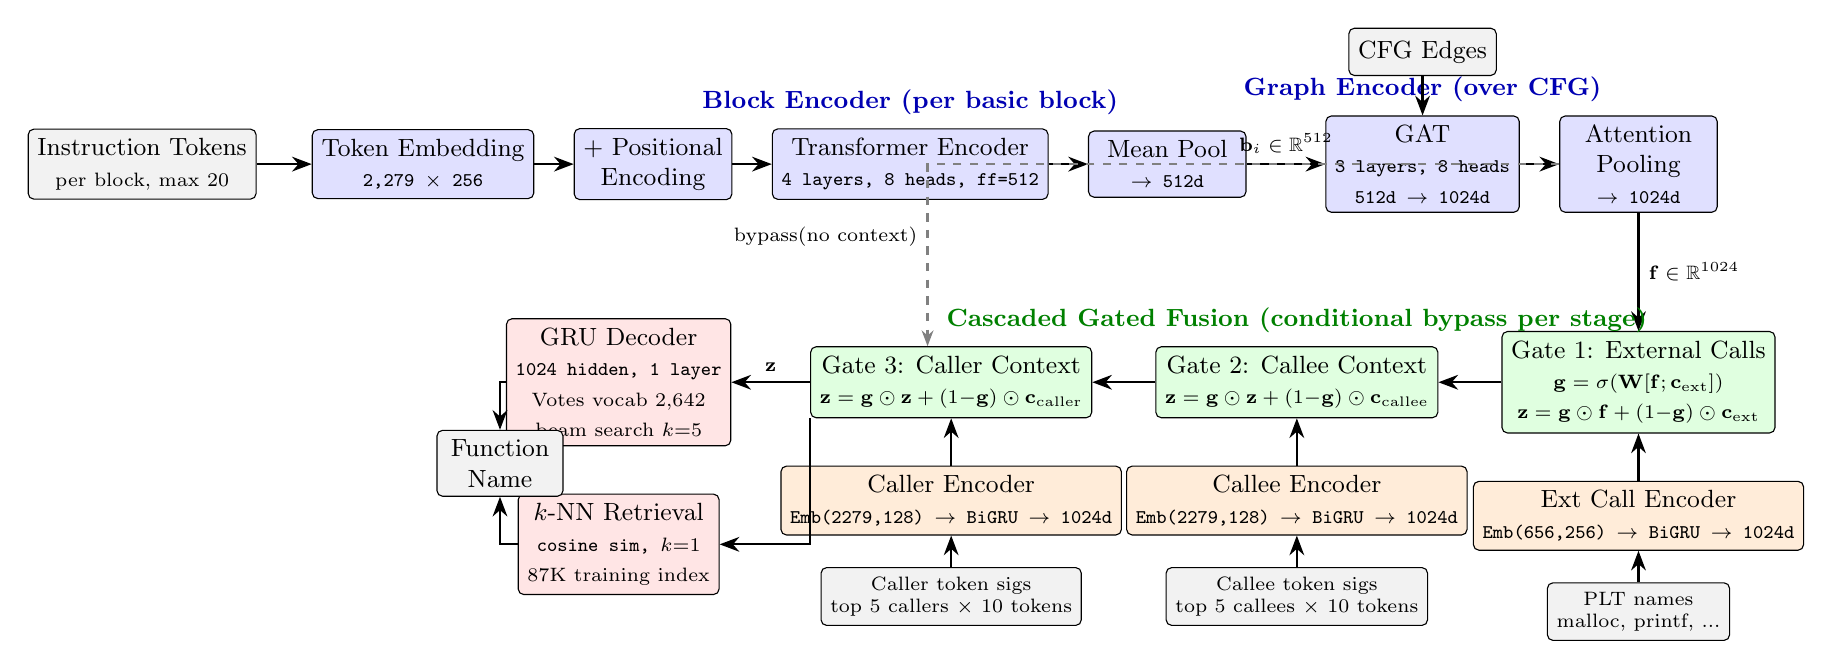
\begin{tikzpicture}[
        node distance=0.5cm and 0.6cm,
        box/.style={rectangle, draw, rounded corners=2pt, minimum height=0.6cm, align=center, font=\small},
        enc/.style={box, fill=blue!12, minimum width=2.0cm},
        ctx/.style={box, fill=orange!15, minimum width=1.8cm},
        gate/.style={box, fill=green!12, minimum width=2.2cm, minimum height=0.8cm},
        dec/.style={box, fill=red!10, minimum width=1.8cm},
        data/.style={box, fill=gray!10, minimum width=1.6cm},
        arr/.style={-{Stealth[length=2.5mm]}, thick},
        byp/.style={-{Stealth[length=2mm]}, thick, dashed, gray},
        lbl/.style={font=\scriptsize, text=black},
    ]

    % ----- Block Encoder -----
    \node[data] (tok) {Instruction Tokens\\{\scriptsize per block, max 20}};
    \node[enc, right=0.7cm of tok] (emb) {Token Embedding\\{\scriptsize\ttfamily2,279 $\times$ 256}};
    \node[enc, right=0.5cm of emb] (pe) {+ Positional\\Encoding};
    \node[enc, right=0.5cm of pe] (txf) {Transformer Encoder\\{\scriptsize\ttfamily4 layers, 8 heads, ff=512}};
    \node[enc, right=0.5cm of txf] (pool) {Mean Pool\\{\scriptsize\ttfamily$\rightarrow$ 512d}};

    \draw[arr] (tok) -- (emb);
    \draw[arr] (emb) -- (pe);
    \draw[arr] (pe) -- (txf);
    \draw[arr] (txf) -- (pool);

    \node[above=0.05cm of txf, font=\small\bfseries, text=blue!70!black] {Block Encoder (per basic block)};

    % ----- Graph Encoder -----
    \node[enc, right=1.0cm of pool] (gat) {GAT\\{\scriptsize\ttfamily3 layers, 8 heads}\\{\scriptsize\ttfamily512d $\rightarrow$ 1024d}};
    \node[enc, right=0.5cm of gat] (attnpool) {Attention\\Pooling\\{\scriptsize\ttfamily$\rightarrow$ 1024d}};

    \draw[arr] (pool) -- node[above, lbl] {$\mathbf{b}_i \in \mathbb{R}^{512}$} (gat);
    \draw[arr] (gat) -- (attnpool);

    \node[above=0.05cm of gat, font=\small\bfseries, text=blue!70!black] {Graph Encoder (over CFG)};
    \node[data, above=0.5cm of gat] (edges) {CFG Edges};
    \draw[arr] (edges) -- (gat);

    % ----- Gated Fusion (vertical layout below) -----
    \node[gate, below=1.5cm of attnpool] (g1) {Gate 1: External Calls\\{\scriptsize $\mathbf{g} = \sigma(\mathbf{W}[\mathbf{f};\mathbf{c}_\text{ext}])$}\\{\scriptsize $\mathbf{z} = \mathbf{g} \odot \mathbf{f} + (1{-}\mathbf{g}) \odot \mathbf{c}_\text{ext}$}};
    \node[gate, left=0.8cm of g1] (g2) {Gate 2: Callee Context\\{\scriptsize $\mathbf{z} = \mathbf{g} \odot \mathbf{z} + (1{-}\mathbf{g}) \odot \mathbf{c}_\text{callee}$}};
    \node[gate, left=0.8cm of g2] (g3) {Gate 3: Caller Context\\{\scriptsize $\mathbf{z} = \mathbf{g} \odot \mathbf{z} + (1{-}\mathbf{g}) \odot \mathbf{c}_\text{caller}$}};

    % Context encoders
    \node[ctx, below=0.6cm of g1] (extenc) {Ext Call Encoder\\{\scriptsize\ttfamily Emb(656,256) $\rightarrow$ BiGRU $\rightarrow$ 1024d}};
    \node[ctx, below=0.6cm of g2] (calleeenc) {Callee Encoder\\{\scriptsize\ttfamily Emb(2279,128) $\rightarrow$ BiGRU $\rightarrow$ 1024d}};
    \node[ctx, below=0.6cm of g3] (callerenc) {Caller Encoder\\{\scriptsize\ttfamily Emb(2279,128) $\rightarrow$ BiGRU $\rightarrow$ 1024d}};

    % Data inputs for context
    \node[data, below=0.4cm of extenc, font=\scriptsize] (extdata) {PLT names\\{\scriptsize malloc, printf, ...}};
    \node[data, below=0.4cm of calleeenc, font=\scriptsize] (calleedata) {Callee token sigs\\{\scriptsize top 5 callees $\times$ 10 tokens}};
    \node[data, below=0.4cm of callerenc, font=\scriptsize] (callerdata) {Caller token sigs\\{\scriptsize top 5 callers $\times$ 10 tokens}};

    \draw[arr] (extdata) -- (extenc);
    \draw[arr] (calleedata) -- (calleeenc);
    \draw[arr] (callerdata) -- (callerenc);
    \draw[arr] (extenc) -- (g1);
    \draw[arr] (calleeenc) -- (g2);
    \draw[arr] (callerenc) -- (g3);

    % Main flow through gates
    \draw[arr] (attnpool.south) -- node[right, lbl] {$\mathbf{f} \in \mathbb{R}^{1024}$} (g1.north);
    \draw[arr] (g1) -- (g2);
    \draw[arr] (g2) -- (g3);

    % Bypass
    \draw[byp] (attnpool.west) -| node[left, lbl, pos=0.7] {bypass\\(no context)} ([xshift=-0.3cm]g3.north);

    \node[above=0.05cm of g2, font=\small\bfseries, text=green!50!black] {Cascaded Gated Fusion (conditional bypass per stage)};

    % ----- Output heads -----
    \node[dec, left=1.0cm of g3] (decoder) {GRU Decoder\\{\scriptsize\ttfamily1024 hidden, 1 layer}\\{\scriptsize Votes vocab 2,642}\\{\scriptsize beam search $k{=}5$}};
    \node[dec, below=0.6cm of decoder] (knn) {$k$-NN Retrieval\\{\scriptsize\ttfamily cosine sim, $k{=}1$}\\{\scriptsize 87K training index}};

    \draw[arr] (g3.west) -- node[above, lbl] {$\mathbf{z}$} (decoder.east);
    \draw[arr] (g3.south west) |- (knn.east);

    \node[data, left=0.7cm of $(decoder)!0.5!(knn)$] (out) {Function\\Name};
    \draw[arr] (decoder.west) -| (out.north);
    \draw[arr] (knn.west) -| (out.south);

    \end{tikzpicture}%

\end{document}
